%
% ---------------------------------------------------
%
% Proyecto de Final de Carrera:
% Author: José Lucas Grillo Lorenzo <jlucas.gl@gmail.com>
% Capítulo: Optimizaciones en GPGPU
% Fichero: Cap5_Opt_GPGPU.tex
%
% ----------------------------------------------------
%

\chapter{Optimizaciones en \gpgpu{}}
\label{chap:optGPGPU}

En este Capítulo se pone de manifiesto la investigación en optimizaciones para
arquitecturas \gpgpu{} usando
el compilador \yacf{}. Una herramienta de compilación \ac{StS} con la 
que el autor ha podido desarrollar algunas técnicas de optimización bien conocidas para 
\gpgpu{} en el marco de la versión 1.0 del estándar \ac{OpenACC}.

% Ecribir sobre \gpgpu{} y el \tiling{} para \gpgpu{}

\section{Arquitecturas \gpu{}s}
\label{sec:arquitecturasGPU}

% Concepto de kernel 
Las \gpu{}s son arquitecturas que explotan el paralelismo a nivel de \thread{}s. En este 
contexto se define un \thread{}, o hilo, como un conjunto de instrucciones simples que han 
de ser ejecutadas de forma independiente y paralela. Estas instrucciones simples están 
definidas en lo que se conoce como \textit{kernel}, que no es más que un código fuente, 
generalmente escrito en un subconjunto de C con extensiones para ser ejecutado por un 
conjunto de \thread{}s en un dispositivo acelerador.

Estos conceptos son habituales para un programador de \CUDA{} y también extensibles a 
\OpenCL{}. Por simplicidad, se tratan ahora algunos aspectos de la arquitectura \CUDA{}. 
La arquitectura de \OpenCL{} es ligeramente distinta pero no se entrarán en esos detalles
diferenciadores al no resultar relevantes.

\subsection{Modelos arquitecturales lógico y hardware: CUDA}

% Describir modelo lógico(CUDA) y hardware
% Añadir imagenes de la arquitectura CUDA
% Describir mínimamente la jerarquía de threads
%%%%%%%%%%%%%%%%%%%%%%%%%%%%%%%%%%%%% Figure %%%%%%%%%%%%%%%%%%%%%%%%%%%%%%%%%%%%%%%%%%%%%
\begin{figure}[!h]
	\centering
	\includegraphics[width=0.8\linewidth]{CUDA_logical.png}
	\caption{Modelo lógico de \CUDA{}}
	\label{fig:CUDAlogical}
\end{figure}
%%%%%%%%%%%%%%%%%%%%%%%%%%%%%%%%%%%%%%%%%%%%%%%%%%%%%%%%%%%%%%%%%%%%%%%%%%%%%%%%%%%%%%%%%%

El modelo teórico de \CUDA{} representado en la Figura \ref{fig:CUDAlogical} asume que se 
dispone de un número infinito de \thread{}s en 
ejecución, pero no garantiza que esos \thread{}s estén ejecutándose a la vez. Si la 
pregunta es cuantos \thread{}s se ejecutarán simultáneamente, la respuesta será que 
esto depende de la arquitectura hardware, no de la lógica. Como el hardware cambia con 
rapidez, la arquitectura lógica intenta simplificar esto
permitiendo a los usuarios definir una partición lógica de \thread{}s y bloques de 
\thread{}s. De esta forma, los \thread{}s dentro de un bloque se ejecutarán 
simultáneamente, mientras que los bloques de \thread{}s pueden ejecutarse a la vez o no,
según lo recursos hardware disponibles. El conjunto de bloques de \thread{}s es lo que se 
denomina \textit{grid}.

%%%%%%%%%%%%%%%%%%%%%%%%%%%%%%%%%%%%% Figure %%%%%%%%%%%%%%%%%%%%%%%%%%%%%%%%%%%%%%%%%%%%%
\begin{figure}[!h]
	\centering
	\includegraphics[width=0.8\linewidth]{SMFermi.png}
	\caption{Diagrama de un \textit{Streaming Multiprocessor} de la arquitectura Fermi de \NVIDIA{}}
	\label{fig:SMFermi}
\end{figure}
%%%%%%%%%%%%%%%%%%%%%%%%%%%%%%%%%%%%%%%%%%%%%%%%%%%%%%%%%%%%%%%%%%%%%%%%%%%%%%%%%%%%%%%%%%

% Describir mínimamente los warps
La unidad mínima de un bloque de \thread{}s, en la arquitectura CUDA, es lo que de conoce 
como \warp{}. Equivale a 32 threads, aunque este número pudiera cambiar en un futuro. Los 
\ac{SM} como el mostrado en la Figura \ref{fig:SMFermi}, crean, gestionan, planifican
y ejecutan los \thread{}s con granularidad de \warp{}, de tal forma que todos los 
\thread{}s de un \warp{} ejecutan la misma instrucción a la vez. Aunque en el caso de que 
aparezcan divergencias condicionales, el \warp{} ejecuta secuencialmente cada una de las 
ramas tomadas.

%Cuando se accede a la memoria global, se trata de que los accesos de los \thread{}s de un 
%warp sean coalescentes, empleando el menor número de transacciones posibles.

\section{El estándar \ac{OpenACC}}

% El modelo de programación para arquitecturas heterogeneas basado en directivas
% Introducción *muy básica* al estándar y descripción mínima de su uso

% Ecribir introducción básica sobre \ac{OpenACC}
El estándar \OpenACC{} v1.0 \cite{URL::OpenACC} define un modelo de programación para 
arquitecturas heterogéneas basado en directivas.
Fue publicado en noviembre de 2011 y ha servido para apoyar todo el 
desarrollo que se venía realizando el grupo \GCAP{} en este campo.

En la primera versión de dicho estándar, se introducen directivas y cláusulas para la 
gestión de códigos orientados a ser 
ejecutados en las \gpu{}s. Así como la gestión de las transferencias de memoria entre 
CPU (\textit{host}) y \gpu{} (dispositivo acelerador),
críticas para una buena implementación en este tipo de arquitecturas.

Como ejemplos de dichas directivas, el estándar introduce \texttt{\#pragma acc data}, que 
mediante cláusulas como \texttt{copyin} o \texttt{copyout}, permite indicar al 
compilador que una lista de variables debe ser transferida respectivamente hacia o desde 
el dispositivo.

En la versión 1.0 de \OpenACC{}, las directivas encargadas de extraer un código a la 
\gpu{} son: \texttt{\#pragma acc kernels} que indica que la siguiente región de código
ha de generar uno o varios kernels en función de los bucles encontrados en dicha región;
y \texttt{\#pragma acc parallel} que indica que la región de código ha de ejecutarse en un
único kernel. 

La directiva \texttt{kernels} no tiene sentido sin marcar los bucles que
deben ser analizados. Para ello, se emplea la cláusula \texttt{loop} que etiqueta el bucle
inmediatamente a continuación de la \texttt{\#pragma} que contiene dicha cláusula.

Por otra parte, y aunque la directiva \texttt{parallel} no depende necesariamente de la 
existencia de bucles en su región, sí es posible etiquetar los bucles dentro de una región 
\texttt{parallel} para indicar así que el espacio de iteraciones de estos bucles debe
ser distribuido entre los \thread{}s disponibles.


\subsection{Sobre gangs y workers en \ac{OpenACC} v1.0}
\label{subsec:gangsworkers}
% Introducir correlación entre gangs/workers y thread-blocks/threads.
% Añadir \ref{sec:arquitecturasGPU}
Como se describe en la Sección \ref{sec:arquitecturasGPU}, en las arquitecturas \gpu{} 
las unidades de cómputo se estructuran en bloques de \thread{}s
de tamaño determinado, y agrupaciones independientes de bloques de \thread{}s en 
\grid{}s.

% Meter la gráfica donde se ve la *fuerte* dependencia de los compiladores actuales de los 
% valores de gang-worker
% Cita al estándar donde se describen gang y worker
El estándar \ac{OpenACC} \cite{URL::OpenACC} introdujo las 
cláusulas \gang{}, \worker{} y \cvector{} para las regiones \texttt{kernels}, y
\texttt{num\_gangs} , \texttt{num\_workers} y \texttt{num\_vectors} para las regiones \texttt{parallel}.
Estas cláusulas tienen como principal objetivo 
dar al programador mayor control sobre la planificación del código que 
se descarga al acelerador.

Aunque el estándar no determina detalles de su implementación,
en el desarrollo de los compiladores recientes en los que se ha abordado la integración de 
\ac{OpenACC}, se han tomado distintas soluciones para las cláusulas que nos ocupan. En 
algunas implementaciones como las seguida por \CAPS{} y la descrita aquí para 
\accULL{}, se ha optado por dar uso a solo dos de estos niveles: \textit{gang}s, 
correspondiente a grupos de bloques; y \textit{worker}s, para determinar el tamaño de 
los bloques de {thread}s. Reservando la cláusula \cvector{} para una futura aplicación
a instrucciones vectoriales \SIMD{} dentro de cada \thread{}.
% jerarquía de \thread{}s, por \grid{} y por bloques de \thread{}s,

Las cláusulas \texttt{num\_Xs} fijan un tamaño de cada nivel de planificación \texttt{X}, 
para las regiones \texttt{parallel} que las contienen. Así, los tamaños de 
\textit{worker}s y \textit{gang}s asignados respectivamente 
a una serie de bucles etiquetados con la cláusula \texttt{loop}, determinarán las 
dimensiones de esta asignación jerárquica de \thread{}s. Es decir, por ejemplo, las 
iteraciones de un bucle etiquetado con \texttt{\#pragma acc loop gang(64) worker(32)} o
una región \texttt{\#pragma acc parallel loop num\_gangs(64) num\_workers(32)},
distribuirán las iteraciones del bucle entre \texttt{64} bloques de \thread{}s, con 
\texttt{32} \thread{}s cada bloque.
% Cláusulas con tamaño fijo vs cláusulas sin tamaño explícito: que el compilador lo determine
También es posible no indicar explícitamente el tamaño de la distribución jerárquica de
threads, dejando así que el compilador la decida.

En definitiva, las cláusulas \gang{}, \worker{} y \cvector{} pueden ayudar al compilador a 
mapear el espacio de iteraciones de los bucles a la arquitectura subyacente.

\subsection{\tiling{} para mapear un espacio de iteraciones}
\label{subsec:tmaping}
% Estructura por bloques de threads y grids de bloques en \gpgpu{}: Su interpretación en 
% las cláusulas
La interpretación de las cláusulas, citadas en la Sección anterior, seguida en \accULL{} 
ha sido una implementación por \textit{tiles}, o bloques de iteraciones. 
Empleando la transformación \tiling{} descrita en la Sección \ref{subsec:LoopTiling},
también conocida como \textit{blocking} multidimensional.

Esta es una optimización bien conocida desde hace varias décadas 
\cite{Wolfe:1987:IST,Wolfe:1989:MIS},
y recientemente ha resurgido como método para mejorar las prestaciones de códigos \CUDA{} 
\cite{BON:ATC:2008} y en general para dispositivo aceleradores.

%Entre otras utilidades, puede aprovecharse para explotar los múltiples niveles 
%jerarquicos de memoria en arquitecturas como las \gpu{}s. Esto se logra reasignando el 
%espacio de iteraciones a las unidades de cómputo (PEs) siguiendo un esquema jeráquico.

% ¿ Porqué usar \tiling{} con estas cláusulas ?
La estrategia adoptada por el compilador de \CAPS{} para \OpenACC{} en la implementación 
de las cláusulas, ha consistido en seguir una variante del \tiling{} en la que se segmenta 
el espacio de iteraciones en bloques de iteraciones, que se asignan en \gpu{} 
a un número determinado de bloques de \thread{}s (número de \gang{}s) y a un número 
determinado de \thread{}s por cada bloque de \thread{}s (número de \worker{}s).
Por último cada \thread{} recorre su \textit{tile}, de iteración en iteración, 
para respetar el espacio de iteraciones original.

En \accULL{} se decidió adoptar una estrategia similar, siguiendo el modelo clásico de 
\tiling{} asignando \textit{tile}s a \thread{}s como se ha descrito. 
%%% TODO: Como de similar: Strip2Mutator (CAPS o PGI)?? por StripMiningMutator (accULL)
En el caso del compilador de PGI para \OpenACC{} la estrategia difiere, ya que considera 
que los \textit{woker}s han de mapeares con los \warp{}s descritos en la Sección 
\ref{sec:arquitecturasGPU}, mientras que es la cláusula \cvector{} es la que mapea a 
\thread{}s. Dejando al usuario programador la elección de \gang{}s y \cvector{} en lugar 
de \gang{}s y \worker{}s implementada por \CAPS{} y \accULL{}.
%En el caso de CAPS y \accULL{}, se reserva la cláusula \texttt{vector} para una 
%implementación de instrucciones vectoriales SIMD, tal como sugiere el estándar
%de OpenACC \ref{URL::OpenACC}.

%%%%%%%%%%%%%%%%%%%%%%%%%%%%%%%%%%%%% Figure %%%%%%%%%%%%%%%%%%%%%%%%%%%%%%%%%%%%%%%%%%%%%
\begin{figure}[h]
   \centering
   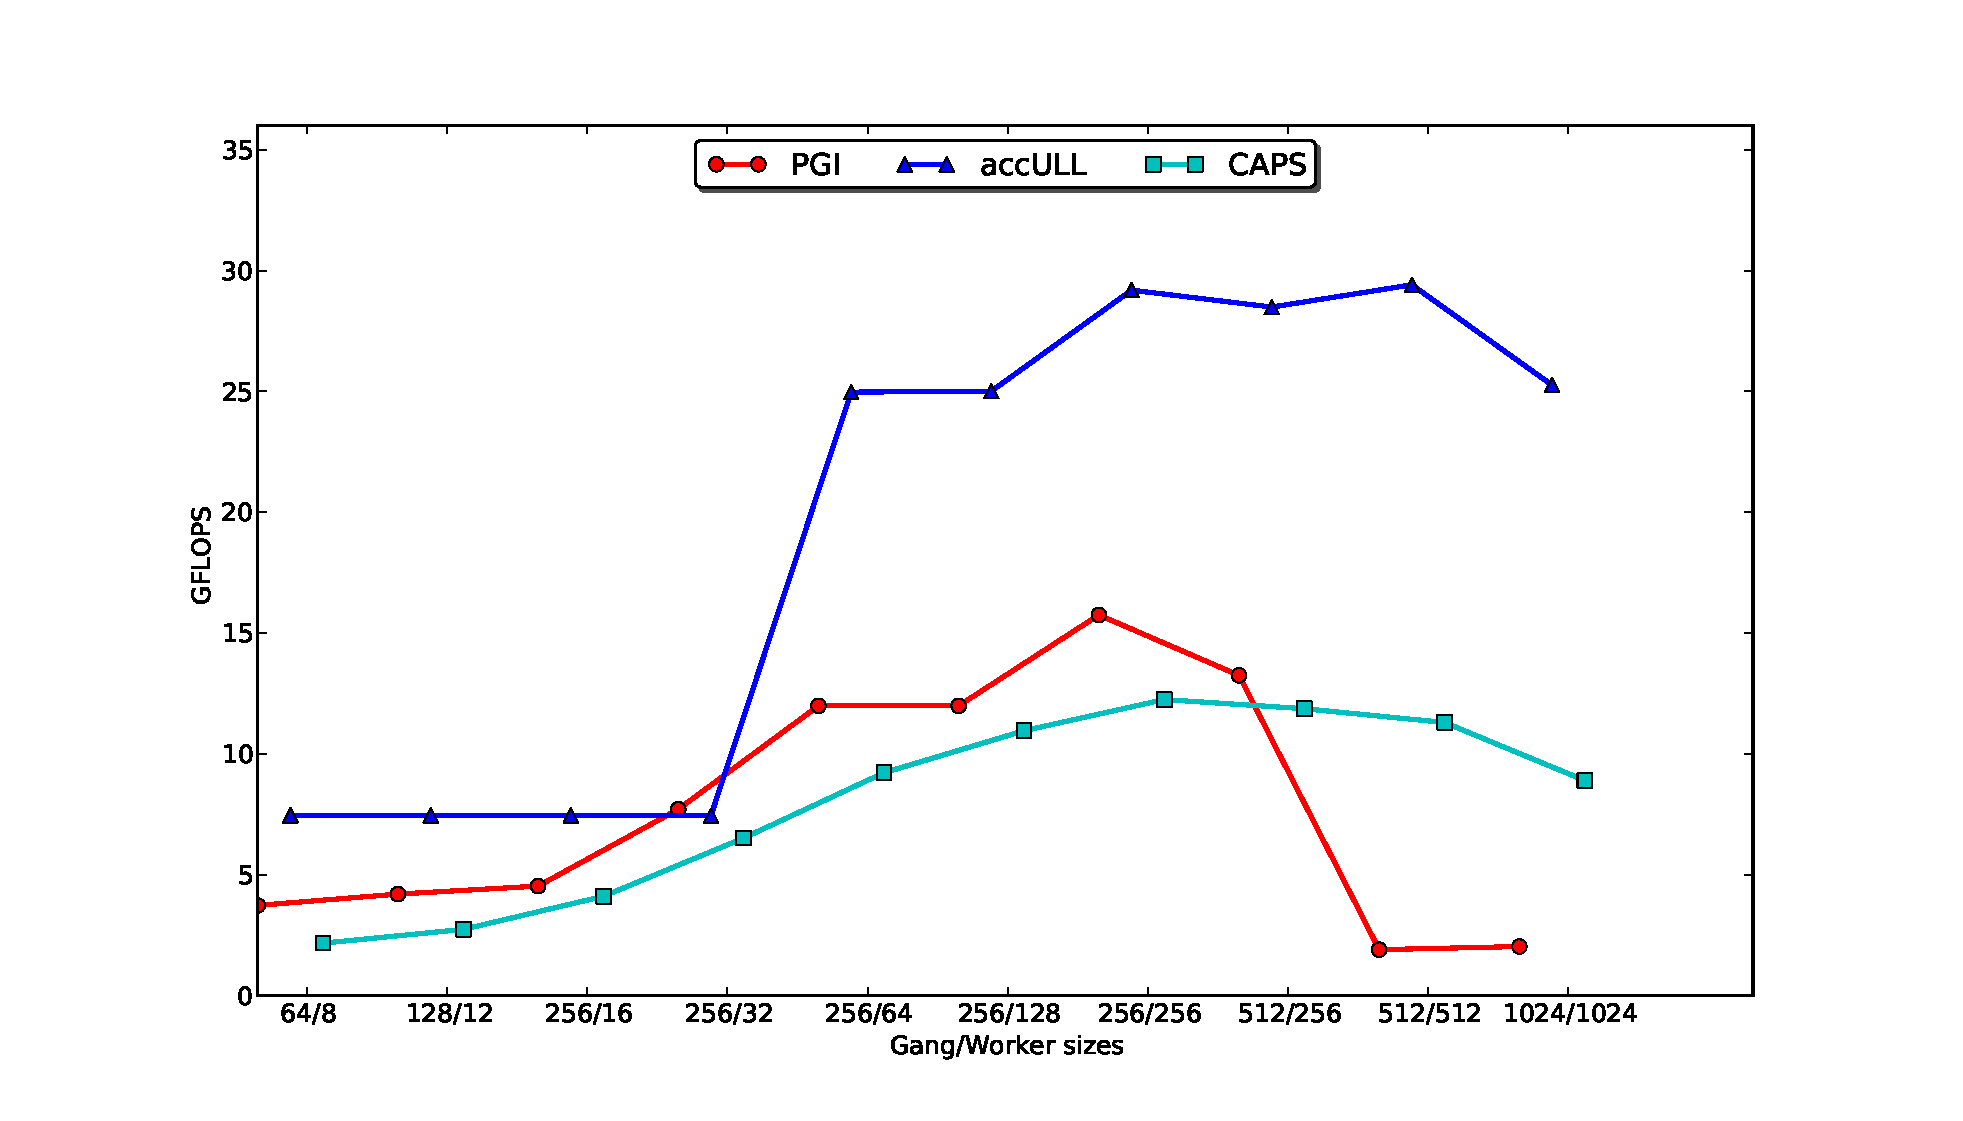
\includegraphics[width=\textwidth]{FIGURES/gemm_flops_varying}
   \caption{Rendimiento de un código evaluado con distintos valores \gang{}/\worker{} para un mismo entorno de ejecución.}
   \label{fig:gemm_gangworker_1}
\end{figure}
%%%%%%%%%%%%%%%%%%%%%%%%%%%%%%%%%%%%%%%%%%%%%%%%%%%%%%%%%%%%%%%%%%%%%%%%%%%%%%%%%%%%%%%%%%

% Revisar resultados del MxM
Los resultados obtenidos en la comparativa de la Figura \ref{fig:gemm_gangworker_1} 
nos hacen pensar que esta interpretación es buena, y puede llegar tomarse como modelo a 
seguir por otros proyectos similares. Se puede deducir una fuerte dependencia de la 
implementación elegida, en la notable 
diferencia entre los resultados mostrados en la Figura \ref{fig:gemm_gangworker_1} al 
ejecutarse un código de multiplicación de matrices etiquetado con \ac{OpenACC} con 
varios compiladores con soporte \OpenACC{} y varios tamaños de \gang{} y \worker{}, o 
\gang{} y \cvector{}.

% Automatizar la generación de una implementación por bloques mediante las cláusulas gang 
% y worker
A continuación se describe el procedimiento seguido para automatizar esta interpretación 
del estándar por bloques.

\section{Mutadores de \yacf{} implicados en la transformación}
\label{sec:mutatorstiling}
%XXX Escribir introducción. Nombrar ASTs y mutadores. Uso amplio de las herramientas 
%desarrolladas en \yacf{}.

Las transformaciones de código intermedio (ver Sección \ref{subsec:IR}) se pueden 
lograr aplicando mutadores (ver Sección \ref{subsec:mutator}) y filtros (ver Sección 
\ref{subsub:filter}) que seleccionen los segmentos del \ac{AST} que ha de ser 
transformado. En este trabajo se ha hecho uso amplio de las herramientas desarrolladas
en \yacf{} como se ha mencionado en la Sección \ref{subsec:loopopt}.

%XXX Escribir sobre el mutador \package{LoopTilingMutator} y su descomposición en los 
%mutadores \package{LoopStripMining} y \package{LoopInterchangeMutator}.

En la Sección \ref{subsec:LoopTiling} se describe en detalle como se descompone el mutador 
\package{LoopTilingMutator} en los mutadores \package{LoopStripMining} y 
\package{LoopInterchangeMutator}, donde se incluye el algoritmo seguido
para este fin (Algoritmo \ref{alg:tiling}).


\subsection{El módulo \package{LoopInterchangeMutator.py}}
Inicialmente este módulo estaba definido como un
intercambiador de dos bucles perfectamente anidados consecutivos, y atendía a las 
cláusulas \llc{} \cite{URL::LLC} heredadas de la investigación llevada a cabo por el grupo
\cite{Garcia:1997:LLC,Luna:1998:HED} \cite{Almeida:2003:PSU,Dorta:2003:LPS}
\cite{Reyes:2011:ACG}. 

Para emplearse y ser realmente útil en la implementación
seguida del \package{LoopTilingMutator} fue necesario remodelarlo completamente. Aunque ha 
quedado en desuso, se ha mantenido la retrocompatibilidad con las cláusulas \llc{} 
originales.

A continuación se detallan los requisitos de este mutador  de cara a la implementación del 
driver descrito en la Sección \ref{chap:optGPGPU:accgangworker}:

\begin{itemize}
\item Dar múltiples opciones al desarrollador de drivers para un uso versátil del mutador 
en el paso de parámetros y establecer un comportamiento por defecto basado en el mutador 
original.
\item Permitir intercambiar dos bucles cualesquiera en un anidamiento perfecto, 
indistintamente de su nivel de profundidad o del orden en el que se le indicase (más 
profundo por menos profundo o viceversa).
\item Asociar a cada bucle las posibles directivas que etiquetasen el bucle.
\end{itemize}

El comportamiento por defecto indicado en el primer punto es el intercambio de los dos 
bucles anidados inmediatamente siguientes al AST suministrado, que es el único parámetro 
requerido en todo mutador. El intercambio flexible de bucles era necesario para su 
integración en el \package{LoopTilingMutator}, ya que es parte del Algoritmo 
\ref{alg:tiling} descrito en la Sección \ref{subsec:LoopTiling}. Por último, era vital
asociar a los bucles intercambiados las posibles pragmas para conservar su significado 
original en el código resultante. Con esto se pretende que las directivas queden en los 
bucles externos al aplicar \tiling{}, y así se puedan paralelizar éstos, enviando a \gpu{} 
los bucles internos. 

%Describir minimamente implementación en cuatro pasos del mutador
El comportamiento de este mutador se describe en detalle en la Sección 
\ref{subsec:interchange}.
%La implementación en cuatro pasos del mutador ... 

\subsection{El módulo \package{LoopStripMiningMutator.py}}

Inicialmente este módulo era la implementación original del \tiling{}. En los ejercicios 
iniciales, la transformación se aplicaba a bucles individuales y no había reordenación, 
con la consecuente falta de coherencia en el resultados del código final.

En la práctica, como se indica en la Sección \ref{subsec:Strip-mining}, aplicar \tiling{} a un único 
bucle es equivalente a aplicar a dicho bucle \textit{Loop Strip-Mining}.
De esta manera, siguiendo nuestra metodología de desarrollo continuo, hemos generalizado 
el código que se describe a continuación:

\begin{itemize}
\item Obtener los parámetros y variables necesarias a partir del \ac{AST} suministrado
\item Generar un nuevo bucle con una nueva variable índice que itere sobre los bloques 
\item Modificar el bucle original para que itere dentro de cada bloque
\item Sustituir el nuevo \ac{AST} por el \ac{AST} original y generar las declaraciones 
necesarias y situarlas justo antes del bucle más externo en el orden adecuado
\end{itemize}

El comportamiento de este mutador se describe en detalle en la Sección \ref{subsec:Strip-mining}. Un ejemplo del resultado de este mutador se puede observar en el Listado \ref{code:looptilingmutator1}
después de aplicarlo al código del Listado \ref{code:looptilingmutator0}. 

\subsection{El módulo \package{LoopTilingMutator.py}}
\label{subsubsec:looptilingmutator}

% Escribir detalles de implementación del Algoritmo \ref{alg:tiling}

Es importante destacar que en la implementación del \package{LoopTilingMutator.py} se ha 
optado por dividir el número de iteraciones de los bucles originales por el número de 
\gang{}s y/o \worker{}s, tal y como se describe en la Sección \ref{subsec:gangsworkers},
asignando el código resultante al tamaño del \textit{tile}, y consiguiendo dividir el 
espacio de iteraciones en el número de \gang{}s y \worker{}s solicitado.

\lstinputlisting[float,language=C,caption={Bucle de 10 iteraciones que asigna el número de 
iteración a un vector del mismo tamaño}, label={code:looptilingmutator0}]
{listings/looptilingmutator0.c} %% LISTING

En el Listado \ref{code:looptilingmutator1} se puede observar como la variable 
\texttt{remain\_i} (línea 4) es la que contiene dicho resultado. En la línea 9 se calcula 
la última iteración del bucle interno, garantizando que no se supera el tamaño original.
El Algoritmo \ref{alg:tiling} y la implementación seguida para este módulo se describe en 
detalle en la Sección \ref{subsec:LoopTiling}.

\lstinputlisting[float,language=C,caption={Código resultante de la aplicación del mutador \package{LoopTilingMutator.py}
al código del Listado \ref{code:looptilingmutator0}},
label={code:looptilingmutator1}]{listings/looptilingmutator1.c} %% LISTING


\subsection{Acerca del \driver{} \textit{accgangworker.py}}
\label{chap:optGPGPU:accgangworker}

%XXX Ecribir descripción

% Descripción del driver accgangworker.py
% Sigue el patrón de drivers desarrollados para yacf
% Pasos de la transformación StS: 
%       FrontEnd ( parseo ), anotación de la IR, ...
%                aplicación de la tranformación a las cláusulas
%                generación de código final ( C + OpenACC )

En el transcurso del trabajo realizado se ha desarrollado un \driver{} siguiendo el 
esquema definido en la Sección \ref{chap:yacf:design}, para el análisis y la verificación 
de la correcta implementación de la transformación seguida para las cláusulas \gang{} y 
\worker{}.

Este \driver{} sigue el modelo de ejecutables definido para \yacf{}. Con un análisis 
inicial en el \package{frontend} \ref{subsec:Frontend}, seguido de las correspondientes 
anotaciones de la \ac{IR} \ref{subsec:IR}, la aplicación de los filtros y mutadores, y por 
último un volcado del código resultante mediante el \writer{} %\ref{subsec:writer}
de \OpenACC{} \ref{subsect:AccWriter}.

La estrategia seguida para aplicar \tiling{} a las cláusulas \gang{} y \worker{} ha sido 
filtrar primero todas las cláusulas \worker{}, aplicar \tiling{}. Por último se filtran 
las cláusulas \worker{} y se aplica el mutador de nuevo.

De esta manera, se consigue segmentar el espacio de iteraciones en cada bloque de threads,
inicialmente usando el número de \worker{}, y posteriormente repitiendo el proceso para 
todo el \grid{}, aplicando la planificación de los \gang{}.

\section{Las regiones \texttt{parallel}}

En la versión 0.3 de \accULL{} se ha añadido soporte para los bucles que se encuentran 
dentro de las regiones \texttt{parallel} - que hasta ahora eran ejecutados 
secuencialmente. 
Para ello se ha implementado un mutador (\class{AccParallelLoopMutator}) que genera código 
capaz de 
distribuir las iteraciones de los bucles entre los \thread{}s/bloques que conforman el 
grid en ejecución. Dicho mutador resuelve la distribución de los bucles anidados mediante 
recursividad. 

\lstinputlisting[float,language=Python,caption={Mutador recursivo AccParallelLoop 
utilizado para la paralelización de las iteraciones dentro de cláusulas 
\texttt{parallel}}, label={code:accparallelloop}]
{listings/accparallelloop.py} %% LISTING

El Listado \ref{code:accparallelloop} muestra una versión simplificada de la 
implementación del mutador. Como se puede observar, en la línea 6 se filtra el \ac{AST}
suministrado buscando la cláusula \texttt{loop}. Una vez obtenida, se extrae el bucle
asociado (línea 8) y éste se parametriza en el diccionario \texttt{loop\_parameters} 
(línea 18). El código interno del bucle se asigna al parámetro \texttt{'code'} dentro del 
diccionario \texttt{system\_parameter}. Ambos diccionarios son aplicados a la plantilla
mostrada en el Listado \ref{code:template_ploop} como \texttt{'l\_p'} y \texttt{'s\_p'} respectivamente, que 
posteriormente es parseada mediante la función heredada \texttt{parse\_snippet} (línea 
25). En la línea 30 se aplica la herramienta \class{ReplaceTool} descrita en la Sección
\ref{subsec:handleIR}, para retirar del \ac{AST} las directivas asociadas al bucle.

Finalmente en la línea 34 se hace una llamada recursiva al mutador. Las líneas 11, 14-15 y 
38 controlan la recursividad del mutador, no permitiendo más de dos niveles de 
anidamiento. Además en ningún momento se aplicarán más niveles de recursividad que bucles
anidados estén etiquetados. Esto se controla al disparar una excepción de tipo 
\texttt{NodeNotFound} cuando no se ha encontrado una cláusula \texttt{loop}, rompiendo así
la recursividad.

\lstinputlisting[float,language=C,caption={Plantilla para el mutador recursivo mostrado en
el Listado \ref{code:accparallelloop}}, label={code:template_ploop}]
{listings/template_ploop.c} %% LISTING

\subsection{Ecuaciones de distribución de iteraciones}
\label{subsec:ecuations}

\lstinputlisting[float,language=C,caption={Bucle etiquetado con la cláusula \texttt{loop} 
dentro de una región \texttt{parallel}}, label={code:ploop}]
{listings/parallel_loop.c} %% LISTING

\lstinputlisting[float,language=C,caption={Código del kernel correspondiente al bucle 
etiquetado en el Listado \ref{code:ploop}, después de aplicar el mutador mostrado en
el Listado \ref{code:accparallelloop}}, label={code:ploop_mutated}]
{listings/parallel_loop.cu} %% LISTING


%Cláusulas numgang y numworker en \ac{OpenACC} v1.0
La plantilla mostrada en el Listado \ref{code:template_ploop} genera una serie de 
ecuaciones en lenguaje C destinadas a distribuir las iteraciones de un bucle entre 
\thread{}s y bloques de \thread{}s tal y como se explicó en la Sección 
\ref{subsec:tmaping}. El mutador recursivo mostrado en el Listado 
\ref{code:accparallelloop} se encarga de transformar un código como el mostrado en
el Listado \ref{code:ploop} a un código interpretable por el kernel como el que se
muestra en el Listado \ref{code:ploop_mutated}.
En las líneas 2-3 del Listado \ref{code:ploop_mutated} se calcula un tamaño de salto 
(\textit{stride}) para las iteraciones entre bloques (\textit{block}s) y dentro de cada 
bloque (\thread{}s). En las líneas 5-6 se calcula el inicio de del \textit{tile}, y el
las líneas 8-9 el final. Las líneas 11-14 del Listado \ref{code:ploop_mutated} recorren el 
tile correspondiente a cada \thread{}.

Cuando aparezcan dos bucles etiquetados con la cláusula \texttt{loop} dentro de una región
\texttt{parallel} se tratará de distribuir las iteraciones en bloques de threads de dos 
dimensiones. La primera dimensión de threads para el primer bucle y la segunda dimensión
para el segundo bucle. Un problema abierto en \accULL{} es contemplar que estas ecuaciones
solo se apliquen cuando el número de iteraciones a distribuir es igual o mayor que el 
número de \thread{}s disponibles en todas las dimensiones aplicables. Actualmente si no 
se da este caso pude suceder que los resultados no sean los esperados al omitir la 
ejecución de algunas iteraciones.
